\chapter{Porovn�n� model�}


\begin{figure}[h]
\begin{tabular}{cc}
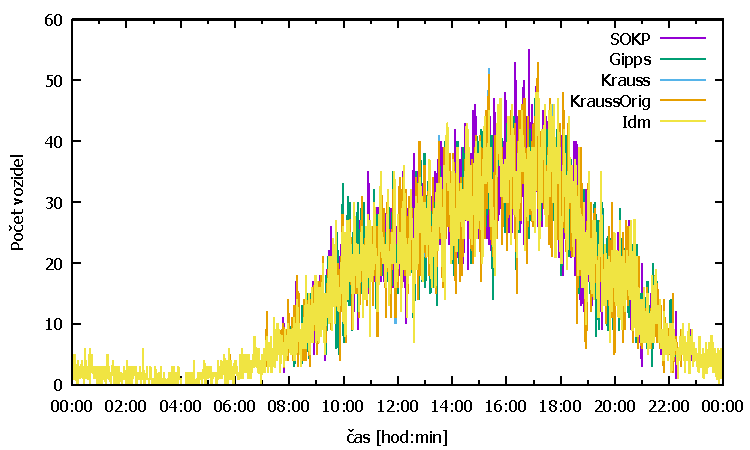
\includegraphics[width=6.5cm]{porovnani/brana218.pdf} & 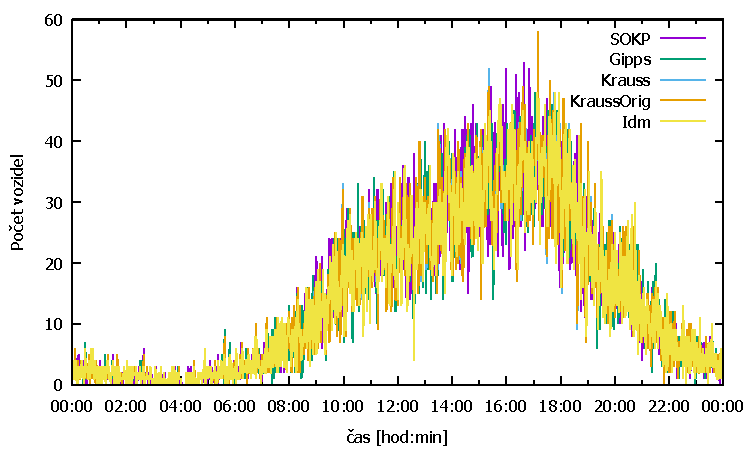
\includegraphics[width=6.5cm]{porovnani/brana201.pdf} \\
a) Br�na 218 & b) Br�na 201 \\
%
\\
%
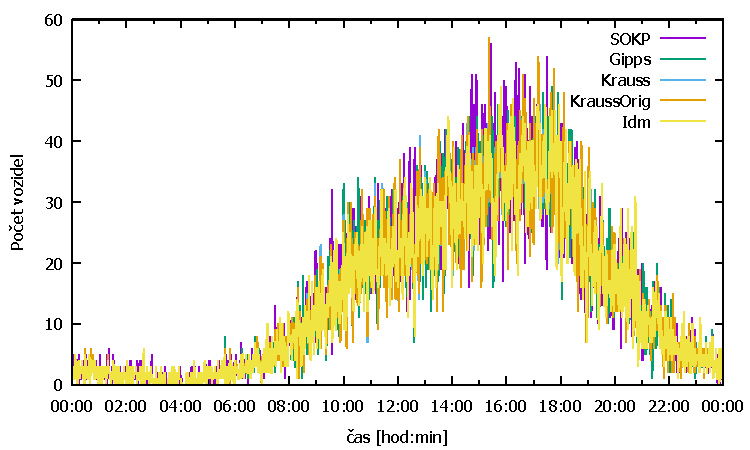
\includegraphics[width=6.5cm]{porovnani/brana187.pdf} & 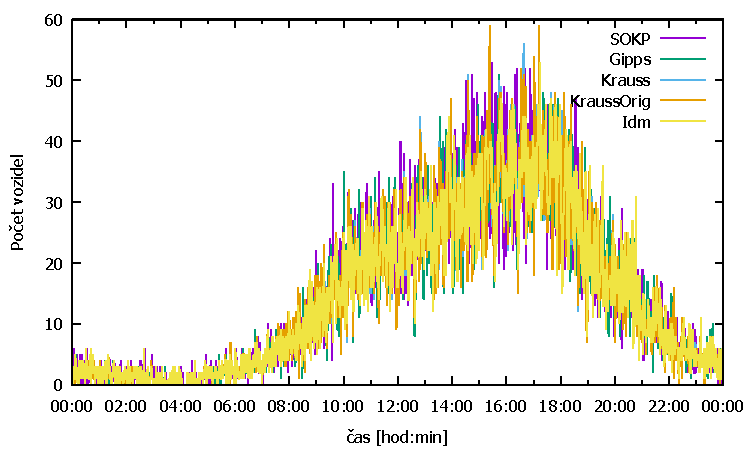
\includegraphics[width=6.5cm]{porovnani/brana170.pdf} \\
c) Br�na 187 & d) Br�na 170
\end{tabular}
\caption{Porovn�n� jednotliv�ch model� mezi sebou - konkr�tn� hodnoty}
\label{fig:porovnanirada}
\end{figure}

\begin{figure}[h]
\begin{tabular}{cc}
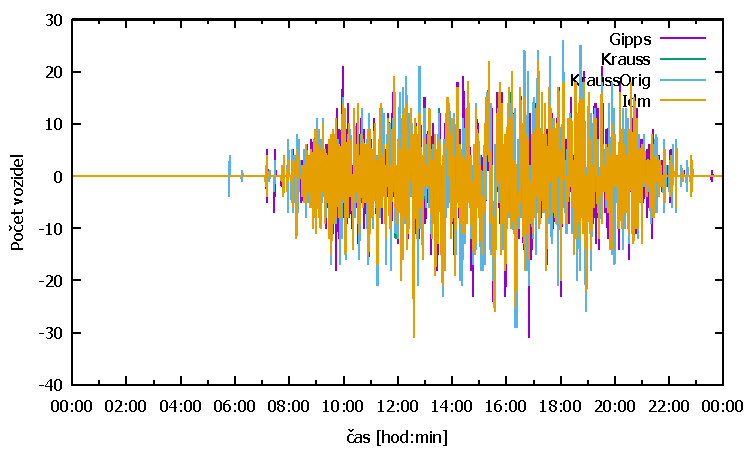
\includegraphics[width=6.5cm]{porovnani/chyba218.pdf} & 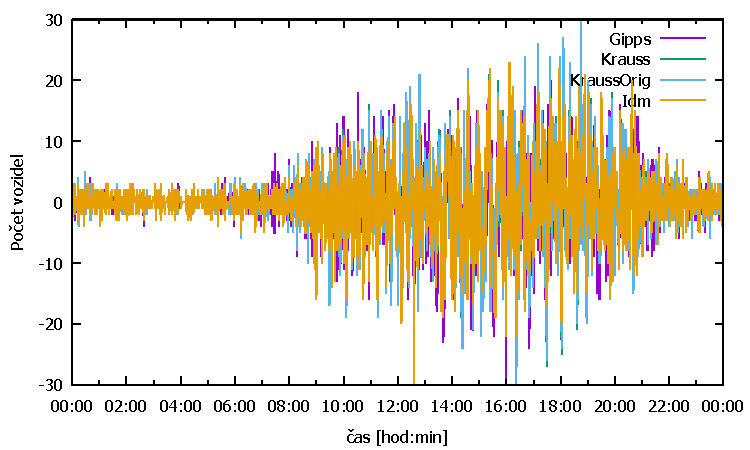
\includegraphics[width=6.5cm]{porovnani/chyba201.pdf} \\
a) Br�na 218 & b) Br�na 201 \\
%
\\
%
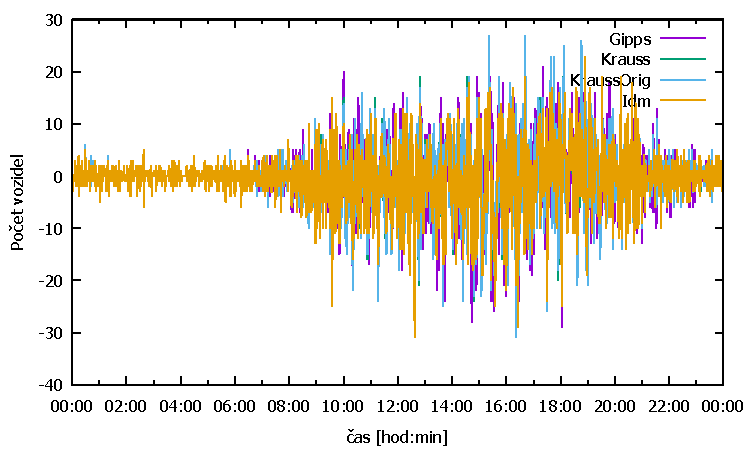
\includegraphics[width=6.5cm]{porovnani/chyba187.pdf} & 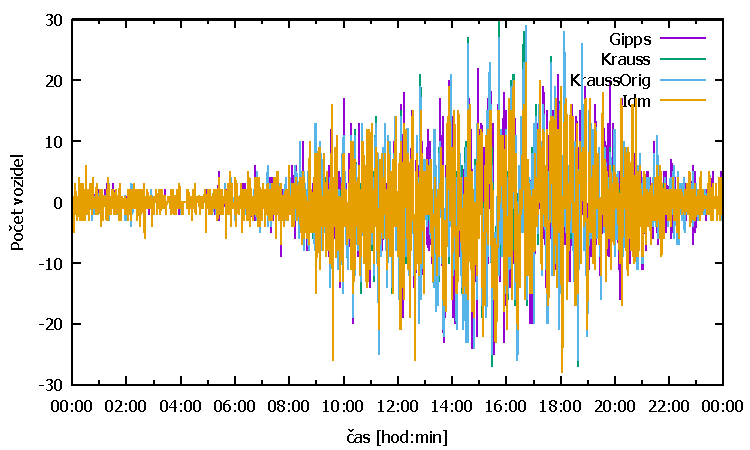
\includegraphics[width=6.5cm]{porovnani/chyba170.pdf} \\
c) Br�na 187 & d) Br�na 170
\end{tabular}
\caption{Porovn�n� jednotliv�ch model� mezi sebou - absolutn� chyby}
\label{porovnanichyba}
\end{figure}

\begin{figure}[h]
\begin{tabular}{cc}
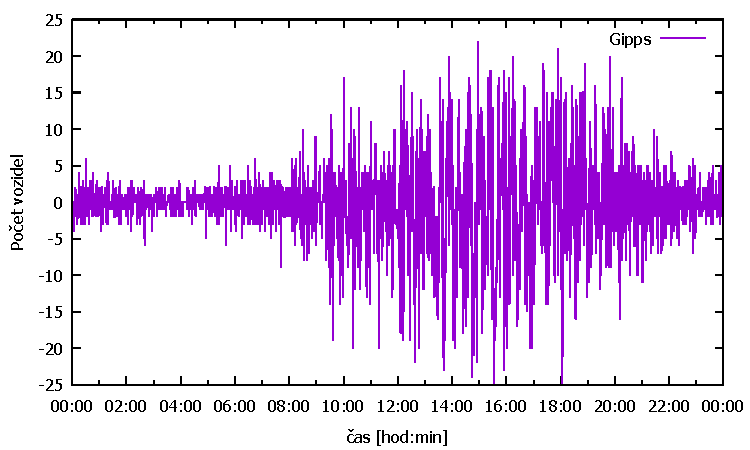
\includegraphics[width=6.5cm]{porovnani/chyba170Gipps.pdf} & 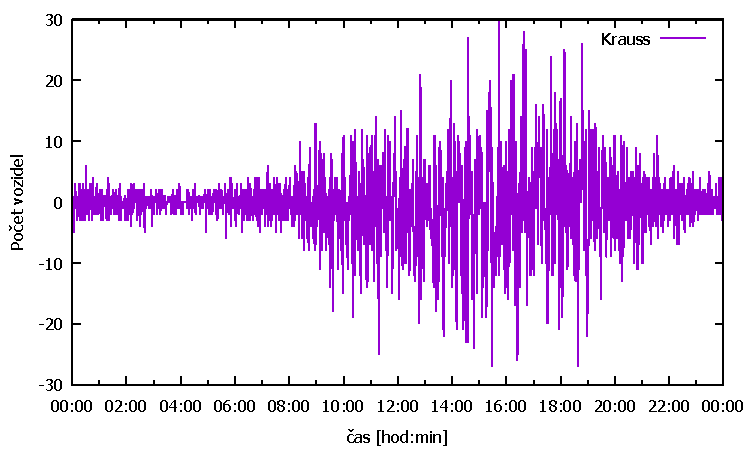
\includegraphics[width=6.5cm]{porovnani/chyba170Krauss.pdf} \\
a) Gipps�v model & b) Krauss�v model \\
%
\\
%
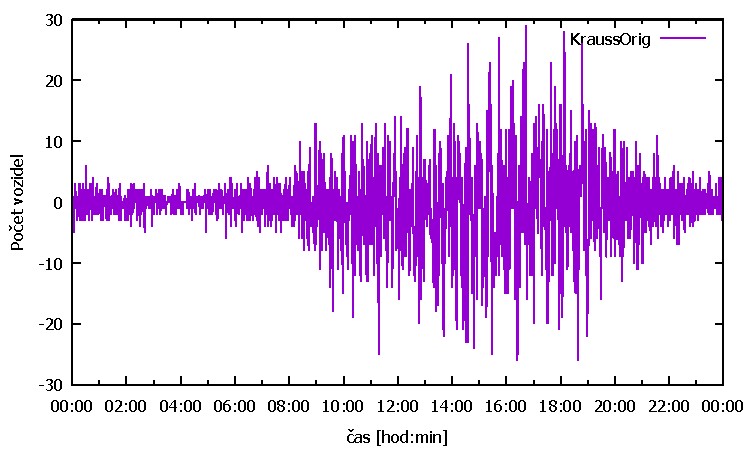
\includegraphics[width=6.5cm]{porovnani/chyba170KraussOrig.pdf} & 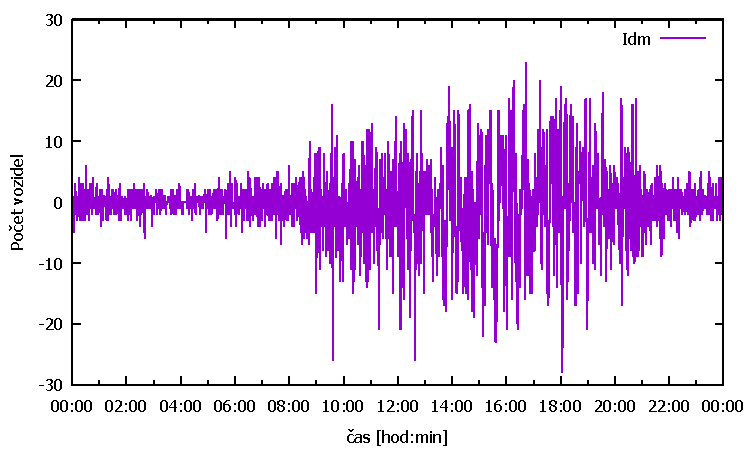
\includegraphics[width=6.5cm]{porovnani/chyba170IDM.pdf} \\
c) Roz���en� Krauss�v model & d) Intelligent Driver Model
\end{tabular}
\caption{Porovn�n� jednotliv�ch model� mezi sebou - m�tn� br�na 0170}
\label{chyba170}
\end{figure}